% Actes EIAH / RJC-EIAH
% S'appuie sur la classe de base llncs,
% avec une gestion de l'utf-8, du français
% Auteurs : Rémi Venant <remi.venant@univ-lemans.fr>, Mathieu Muratet <mathieu.muratet@lip6.fr>
% Version 1.20 - 2024/06/10
%

%%%%%%%%%%%%%%%%%%%%%%%%%%%%%%%%%%%%%%%%%%%%%%%%%%%%%%
%% INCLUSION DES PACKAGES                           %%
%%%%%%%%%%%%%%%%%%%%%%%%%%%%%%%%%%%%%%%%%%%%%%%%%%%%%%
\documentclass[runningheads]{llncs}
\usepackage[utf8]{inputenc} %gestion des fichiers utf8
\PassOptionsToPackage{french}{babel}
\usepackage{babel}
\usepackage[T1]{fontenc}
\usepackage{hyphenat}
\usepackage{subcaption}
\usepackage{graphicx}
\usepackage[dvipsnames]{xcolor}
\usepackage{sectsty}
\usepackage{wrapfig}
\usepackage[titles]{tocloft}
\usepackage{ifthen}
\usepackage{pdfpages}
\usepackage{geometry}
\usepackage[export]{adjustbox}
\usepackage{tocloft}
\usepackage{blindtext}
\usepackage{imakeidx}

% Métadonnées du document pdf généré. 
% pdfauthor: à changer, les auteurs des actes
% pdftitle: à changer, le titre des actes
% pdfsubject: changement optionnel, la "thématique" du document
% pdfproducer: ne pas changer normalement (le logiciel producteur du document)
% pdfcreate: ne pas changer normalement (le logiciel en charge de la création du document pdf)
\usepackage[hidelinks,
pdfauthor={Sonian Mandin et Mathieu Muratet},
pdftitle={Rencontres Jeunes Chercheuses et Chercheurs en EIAH 2024, Laval},
pdfsubject={Actes de conférence},
pdfkeywords={Some Keywords},
pdfproducer={Latex with hyperref},
pdfcreator={pdflatex}]{hyperref}

%%%%%%%%%%%%%%%%%%%%%%%%%%%%%%%%%%%%%%%%%%%%%%%%%%%%%%
%% DEFINITIONS GENERALES - A APADATER SELON CONF    %%
%%%%%%%%%%%%%%%%%%%%%%%%%%%%%%%%%%%%%%%%%%%%%%%%%%%%%%

% Couleur principale du manuscript (utilisée notamment pour les titres principaux)
\definecolor{ConfColor}{HTML}{C30065}

% En-têtes des pages paires/impaires (hors articles)
\newcommand{\proceedingsHeadings}{
	\markboth{Sonian Mandin et Mathieu Muratet}{Rencontres Jeunes Chercheuses et Chercheurs en EIAH 2024, Laval}
}

% Logo de la conférence
\newcommand{\logoConf}[1][0.6]{
	\begin{figure}[h]
		\centering
		
\includegraphics[width=0.4\textwidth]{Content/figures/logoConf.png}
	\end{figure}
}

%%%%%%%%%%%%%%%%%%%%%%%%%%%%%%%%%%%%%%%%%%%%%%%%%%%%%%%%%%%%%
%% DEFINITION DE COMMANDES (MODIFICATIONS NON REOMMANDEES) %%
%%%%%%%%%%%%%%%%%%%%%%%%%%%%%%%%%%%%%%%%%%%%%%%%%%%%%%%%%%%%%

% Redéfinition de mots usuels
\renewcommand\keywordname{{\bf Mots-cl\'es :}}
\addto\captionsfrench{\renewcommand{\figurename}{\upshape Fig.}}
% Définition du formatage des titres, page blanche
\makeatletter
\renewcommand{\@seccntformat}[1]{}
\makeatother
\sectionfont{\LARGE\centering\color{ConfColor}}
\renewcommand{\contentsname}{Table of contents}
\renewcommand{\cftsecfont}{\normalfont\bfseries\color{ConfColor}}% titles in bold
\renewcommand{\cftsecpagefont}{\normalfont\bfseries\color{ConfColor}}% page numbers in bold
\renewcommand{\cftdotsep}{1}
\renewcommand{\cftsecleader}{\bfseries\color{ConfColor}\cftdotfill{\cftsecdotsep}}% dot leaders in bold
\renewcommand{\cftbeforesecskip}{10pt}
\newcommand{\pageblanche}[1][]{
	\newpage
	\ifthenelse{\equal{#1}{}}{
	}{
		\thispagestyle{#1}
	}
	\mbox{}
	\newpage
}
% Assure de faire commencer le prochain contenu sur une page impaire
% Si une page blanche est insérée, celle-ci n'aura aucun en-tête
\newcommand{\startOnOddPage}{
    \ifodd\value{page}
    \else
        \pageblanche[empty]{}
    \fi
}
% Assure de faire commencer le prochain contenu sur une page paire
% Si une page blanche est insérée, celle-ci n'aura aucun en-tête
\newcommand{\startOnEvenPage}{
    \ifodd\value{page}
        \pageblanche[empty]{}
    \else
    \fi
}

\newcommand{\pageTitreSession}[2][]{%
	% Retour au en-têtes des actes
	\proceedingsHeadings
    % La page de titre doit être une page impaire
    \startOnOddPage
	\hspace{0pt}
	\vfill
	\logoConf[0.8]
	\section{#2}
	\ifthenelse{\equal{#1}{}}{
	}{
		\centerline{\large\textbf{#1}}
	}
	\vfill
	\hspace{0pt}
	\newpage
}

% Afficher une liste d'auteurs en limitant possiblement l'affichage au premier avec le suffixe et al. si le nombre  dépasse 3.
% Sinon affiche tous les auteurs, séparés par des virugle sauf pour le dernier, séparé avec un "et".
% 1 - la liste d'auteurs (séparés par des virgules sans espace). Peut être un singleton
\ExplSyntaxOn % nécessaire pour utiliser expl3
\newcommand{\printAuthors}[1]{
	% Le second paramètre (3) fixe le nombre maximal d'auteurs avant d'utiliser la forme compacte
	\internal_print_authors:nn{#1}{3}
}

% Génère une ligne de TOC pour un article et ses auteurs
% 1 - auteurs (séparés par des virgule si plusieurs)
% 2 - titre long de l'article
\newcommand{\paperTitleTocHeading}[2]{
	#2 \newline \textit{\internal_print_authors:n{#1}}
}

\newcommand{\addAuthorsToIndex}[1]{
	\internal_add_authors_to_index:n{#1}
}

% Fonction interne de génération d'une liste formatée d'auteur
% 1 - liste d'auteurs (séparés par des virgule sans espace)
% 2 - nombre maximal d'auteur avant d'utiliser la forme compacte "1er auteur et al."
\cs_new_protected:Nn \internal_print_authors:nn {
	% Définition des variables liste d'auteur (liste) et nombre max d'auteurs (int)
	\clist_set:Nn \l_authors { #1 }
	\tl_set:Nn \l_max_authors { #2 }
	
	\int_compare:nTF { \l_max_authors > 0 } {
		\int_compare:nTF { \clist_count:N \l_authors > \l_max_authors } {
			% Affichage compact: 1er auteur "et al."
			\clist_item:Nn \l_authors { 1 }~et~al.
		} {
			% Liste complète d'auteur séparés par des virgule et un "et" pour le dernier
			\clist_use:Nnnn \l_authors {~et~} {,~} {~et~}
		}
	} {
		% Liste complète d'auteur séparés par des virgule et un "et" pour le dernier
		\clist_use:Nnnn \l_authors {~et~} {,~} {~et~}
	}
}

% Version simplifiée de la fonction avec comme valeur max d'auteurs 0 (desactive le compactage)
\cs_new_protected:Nn \internal_print_authors:n {
	\internal_print_authors:nn {#1} {0}
}

% Pour chaque auteur d'une liste donnée, créer un enregistrement dans l'index
\cs_new_protected:Nn \internal_add_authors_to_index:n {
	\clist_set:Nn \l_authors { #1 }
	\clist_map_variable:NNn  \l_authors \l_author {
		\index{ \l_author}
	}
}
\ExplSyntaxOff

% Fonction interne de génération

% Ajoute un nouvel article aux actes
% les 5 paramètres sont :
%  1 - Auteur(s) (si plusieurs, les séparer par des virgules sans espaces), formatés pour la Toc et les en-têtes (ex.: Prénom Nom)
%  2 - le titre court
%  3 - le titre long
%  4 - l'id
%  5 - le chemin du pdf
% 6 - Auteurs formatés pour l'index (ex.: Nom Prénom)
% Exemple : \addpaper{Nom}{TitreCourt}{TitreLong}{ID}{pdfPath}
\newcommand{\addpaper}[6]{
    % la première page de l'article doit commencer sur une page paire
    \startOnEvenPage
    \addAuthorsToIndex{#6}
    \includepdf[pages={-}, pagecommand={\markboth{\printAuthors{#1}}{#2}}, fitpaper=false, addtotoc={1, subsection, 2, \protect\paperTitleTocHeading{#1}{#3}, #4}]{#5}
    
}

%%%%%%%%%%%%%%%%%%%%%%%%%%%%%%%%%%%%%%%%%%%%%%%%%%%%%%
%% DOCUMENT DES ACTES - A APADATER SELON CONF       %%
%%%%%%%%%%%%%%%%%%%%%%%%%%%%%%%%%%%%%%%%%%%%%%%%%%%%%%

% Gestion de l'index des auteurs
\indexsetup{level=\section,firstpagestyle=myheadings,noclearpage}
\makeindex[title=Index des auteurs,options= -s index_style.ist] % Initialisation de l'index des auteurs

\begin{document}
\pagestyle{myheadings}
\proceedingsHeadings

% Titre des actes
\title{Rencontres Jeunes Chercheuses et Chercheurs en EIAH 2024, Laval}

% Auteurs des actes
\author{Sonia Mandin \and Mathieu Muratet}
\authorrunning{Sonia Mandin \and Mathieu Muratet}

%%%%%%%%%%%%%%%% Page de garde et page blanche %%%%%%%%%%%%%%%%%%%%%%%%%%%%
\thispagestyle{empty}
%\newgeometry{left=3cm,bottom=0.1cm}
\newgeometry{bottom=1cm,top=1cm}

\logoConf[0.7]
\vspace*{2em}
\begin{center}
	\Huge{Actes des dixièmes rencontres jeunes chercheuses et chercheurs en EIAH}
	%{\fontsize{30pt}{36pt}\selectfont Actes des neuvièmes rencontres jeunes chercheurs en EIAH}
	\vspace{0.4em}
	
	\Large{\textit{Environnements Informatiques pour l'Apprentissage Humain}}
\end{center}

\begin{figure}[!ht]
	\centering
		\includegraphics[width=0.62\textwidth]{Content/figures/wordcloud.png}
\end{figure}

\begin{center}
	\begin{Large}
		Édités par Sonia Mandin et Mathieu Muratet
	\end{Large}

	\begin{large}
		Du 4 au 7 juin 2024\\
		Le Mans Université, Laval\\
		France
	\end{large}
\end{center}

\vspace*{\fill}

\begin{figure}[!ht]
	\centering
	\includegraphics[width=.15\textwidth,valign=m]{Content/figures/atief.png}\hfill
	
\includegraphics[width=.3\textwidth,valign=m]{Content/figures/lium_logo.png}\hfill
	
\includegraphics[width=.22\textwidth,valign=m]{Content/figures/cren_logo.jpg}\hfill
	
\includegraphics[width=.18\textwidth,valign=m]{Content/figures/logo_msh.png}\hfill
	
\includegraphics[width=.08\textwidth,valign=m]{Content/figures/logo_LIP6.png}\hfill
\end{figure}

\noindent Avec le soutien de

\begin{figure}[!ht]
	\centering
	
\includegraphics[width=.15\textwidth,valign=m]{Content/figures/lemans_logo.jpg}\hfill
	
\includegraphics[width=.3\textwidth,valign=m]{Content/figures/lium_logo.png}\hfill
	
\includegraphics[width=.15\textwidth,valign=m]{Content/figures/logo_iut.png}\hfill
	
\includegraphics[width=.22\textwidth,valign=m]{Content/figures/cren_logo.jpg}\hfill
	
\includegraphics[width=.15\textwidth,valign=m]{Content/figures/mayenne_logo.png}\hfill
\end{figure}

\begin{center}
	\small{Les dixièmes rencontres jeunes chercheuses et chercheurs en EIAH 2024 ont été organisées}
 
    \small{par Le Mans Université}
    
    \small{sous l’égide de l’ATIEF (Association des Technologies de l’Information pour l’Éducation et la Formation)}
\end{center}

\restoregeometry
\newpage %p1 page de garde

%%%%%%%%%%%%%%%% Table des matière %%%%%%%%%%%%%%%%%%%%%%%%%%%%
\startOnOddPage % Faire commencer la table des matières sur une page impaire
\setcounter{secnumdepth}{1}
\setcounter{tocdepth}{2}
\clearpage
\tableofcontents


%%%%%%%%%%%%%%%% Comités %%%%%%%%%%%%%%%%%%%%%%%%%%%%
\startOnOddPage % Faire commencer la première page des commités sur une page impaire
\vspace*{2em} % permet d'aligner verticalement le titre de la section avec celui de la page de droite (puisque logo placé au dessus de l'introduction)
\section{Comités}
\subsection*{Comité de programme}

\subsubsection*{Présidents :}

\begin{itemize}
	\item[] Sonia Mandin, Université Grenoble-Alpes - MSH-Alpes
	\item[] Mathieu Muratet, INSEI - LIP6 (Sorbonne Université)
\end{itemize}

\subsubsection*{Membres :}

\begin{itemize}
	\item[] Franck Amadieu, Université de Toulouse - CLLE UMR5263
	\item[] Goumi Antonine,Université Paris Nanterre -  Laboratoire Fonctionnement et Dysfonctionnement Cognitifs (DysCo)
	\item[] Francine Athias, ELLIADD-FR EDUC
	\item[] Vincent Barré, Le Mans Université - LIUM
	\item[] Catherine Bonnat, Haute Ecole pédagogique du canton de Vaud
	\item[] François Bouchet, Sorbonne Université - LIP6
	\item[] Julien Broisin, Université Toulouse 3 Paul Sabatier - IRIT
	\item[] Armelle Brun, Université de Lorraine - LORIA
	\item[] Aillerie Carine, Université de Poitiers
	\item[] Pierre-André Caron, Université de Lille1 - laboratoire CIREL
	\item[] Thibault Carron, Université Savoie Mont Blanc - LIP6
	\item[] Ronan Champagnat, Universite de La Rochelle - L3i
	\item[] Olivier Champalle, LIRIS
	\item[] Salomé Cojean, Université Grenoble Alpes
	\item[] Raphaëlle Crétin-Pirolli, Le Mans Université - CREN
	\item[] Philippe Dessus, Univ. Grenoble Alpes - LaRAC
	\item[] Sébastien George, Le Mans Université - LIUM
	\item[] Jean-Marie Gilliot, IMT Atlantique - Lab-STICC
	\item[] Isabelle Girault, Université de Grenoble Alpes
	\item[] Olivier Grugier, Sorbonne Université, INSPE de Paris - EDA, Université de Paris
	\item[] Cédric Fluckiger, Université Lille 3
	\item[] Ludovic Hamon, Le Mans Université
	\item[] Stéphanie Jean-Daubias, Université de Lyon - LIRIS
	\item[] Sébastien Jolivet, Université de Genève - IUFE \& TECFA
	\item[] Alexis Lebis, IMT Nord Europe
	\item[] Marie Levevre, Université Lyon 1 - LIRIS
	\item[] Domitile Lourdeaux, CNRS
	\item[] Nadine Mandran, Université Grenoble Alpes - Laboratoire d'Informatique de Grenoble (LIG)
	\item[] Bertrand Marne, Le Mans Université - LIUM
	\item[] Christine Michel, Université de Poitiers - Techne
	\item[] Najoua Mohib LISEC, Université de Strasbourg
	\item[] Gaëlle Molinari, Université de Genève, Formation Universitaire à Distance Suisse (Unidistance) - TECFA
	\item[] Sandra Nogry, Université Cergy-Pontoise - Laboratoire Paragraphe
	\item[] Sophie Othman, Université de Franche-Comté
	\item[] Chrysta Pélissier, Université de Montpellier 3 - LHUMAIN 
	\item[] Claudine Piau-Toffolon, Université du Mans
	\item[] Fabrice Pirolli, Le Mans Université
	\item[] Franck Poirier, Université Bretagne-Sud
	\item[] Issam Rebai, IMT Atlantique
	\item[] Christophe Reffay, Université de Franche-Comté
	\item[] Eric Sanchez, Université de Genève
	\item[] Franck Silvestre, Université Toulouse Capitole, IRIT
	\item[] Lucile Vadcard Larac, Université Grenoble Alpes
	\item[] Rémi Venant, Le Mans Université - LIUM
	\item[] Mathieu Vermeulen, Université de Lille - IMT Nord Europe
\end{itemize}

\subsection*{Coordinateurs des ateliers et symposia : }

\begin{itemize}
	\item[]Erika Godde, Université de Bourgogne - LEAD
	\item[]Pierre Laforcade, Le Mans Université - LIUM
\end{itemize}

\subsection*{Comité d'organisation :}

\subsubsection*{Présidents :}

\begin{itemize}
	\item[] Bertrand Marne, Le Mans Université - LIUM
	\item[] Raphaëlle Pirolli, Le Mans Université - CREN
\end{itemize}

\subsubsection*{Membres :}

\begin{itemize}
    \item[] Emma Salin, chargée de communication et de projet, stagiaire en BUT MMI - IUT Laval
    \item[] Mohamed Amine Abrache, Le Mans Université - LIUM
    \item[] Thierry Forest, Le Mans Université - LIUM
    \item[] Mohamed Nail Hefied, Le Mans Université - LIUM
    \item[] Bérénice Lemoine, Le Mans Université - LIUM
    \item[] Mamoudou Ndiaye,  Le Mans Université - CREN
    \item[] Fabrice Pirolli, Le Mans Université - CREN 
\end{itemize}
\newpage

%%%%%%%%%%%%%%%% Introduction %%%%%%%%%%%%%%%%%%%%%%%%%%%%
\startOnOddPage % Faire commencer la première page de l'introduction sur une page impaire
\logoConf % replace le logo de la conf au dessus du titre de la section
\section{Introduction aux actes}
Les dixièmes Rencontres Jeunes Chercheuses et Chercheurs en EIAH (RJC EIAH 2024) se sont tenues à Laval du 4 au 7 juin 2024. Ces rencontres sont une occasion particulièrement importante pour les jeunes chercheuses et chercheurs de la communauté EIAH (Environnements Informatiques pour l’Apprentissage Humain) de pouvoir se rencontrer et échanger avec des chercheuses et chercheurs autour de leurs travaux. 

En effet, les RJC EIAH, organisées tous les 2 ans sous l’égide de l’ATIEF (Association des Technologies de l'Information pour l'Éducation et la Formation) visent le développement de la communauté EIAH par la formation des doctorantes et doctorants issus des différentes disciplines inhérentes au domaine des EIAH et la diffusion de leurs travaux. 

\begin{figure}[!h]
	\centering
	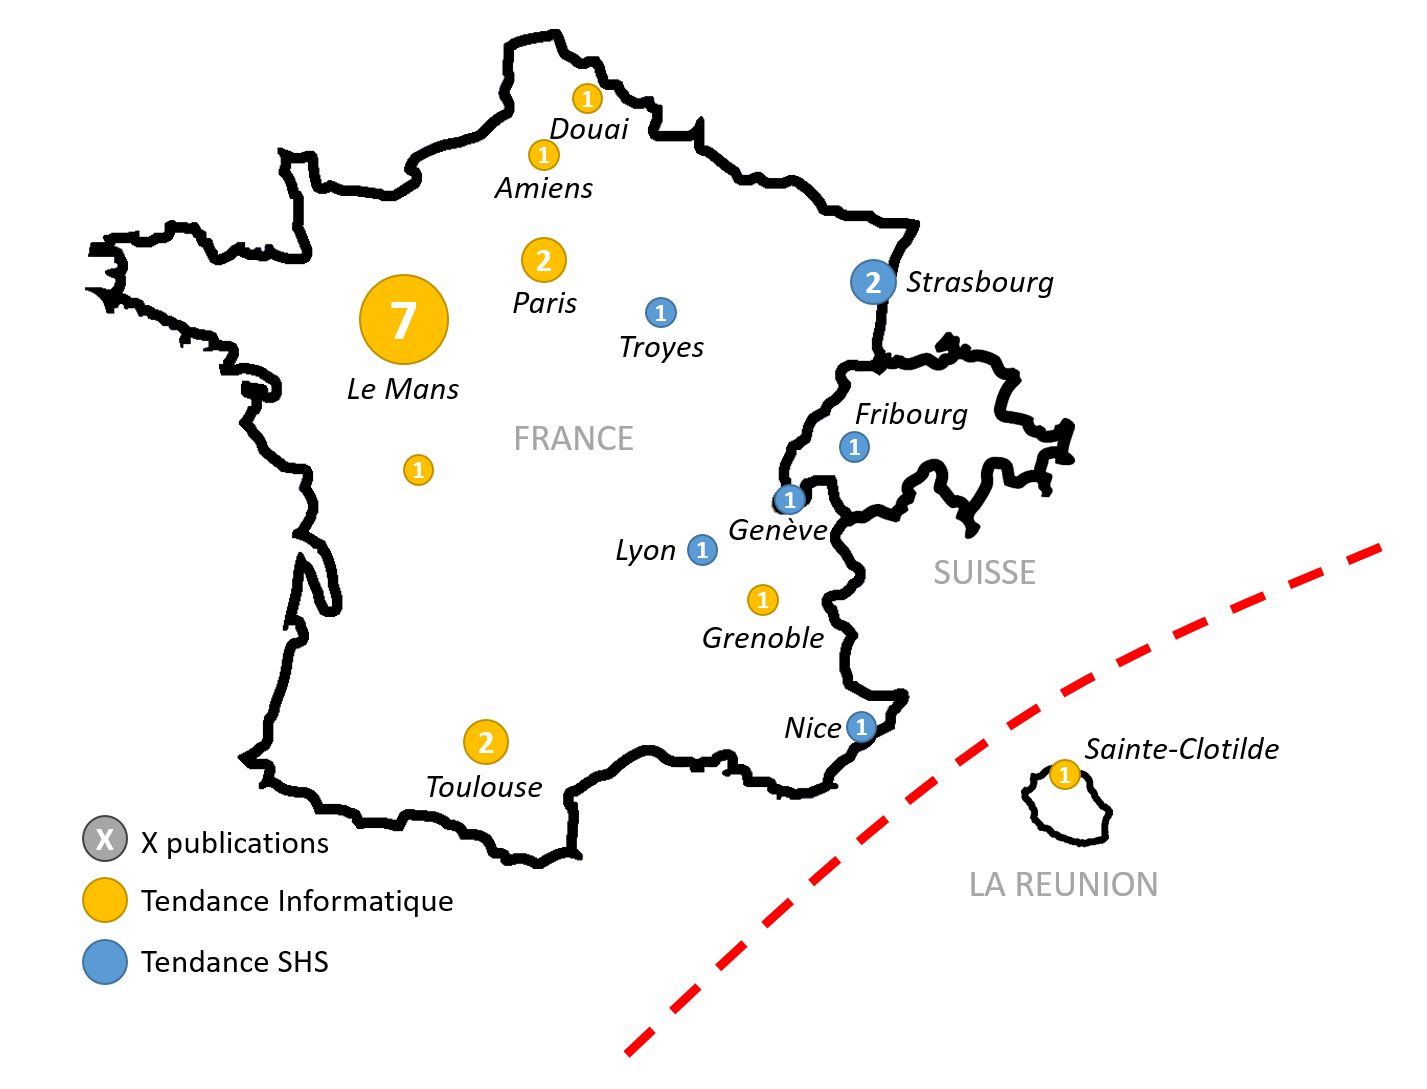
\includegraphics[width=0.7\textwidth]{Content/figures/carteComplete.png}
	\caption{Répartition géographique des publications des RJC EIAH 2024}
	\label{f:repGeoPubli}
\end{figure}

L’édition 2024 a retenu l’attention de 24 jeunes chercheuses et chercheurs qui ont soumis une contribution sous forme d’articles longs de 12 pages pour 17 d’entre eux, et d'articles courts de 4 pages pour 7 autres. 
Chacune des communications ont été évaluées par 2 membres du comité de programme issus pour l'un des sciences humaines et sociales (SHS) et pour l'autre de l'informatique. À l’issue de cette phase d'évaluation, 14 propositions ont été acceptées sous la forme d’articles longs, et 9 ont été acceptées sous la forme d’articles courts. Nous remercions d'ailleurs le comité de programme pour la qualité  des relectures et les commentaires conséquents et pédagogiques qui permettent l’amélioration des articles proposés et des présentations lors de la conférence.

Les articles longs acceptés ont été présentés lors de la conférence sous la forme d'une présentation orale et les articles courts à travers une présentation de poster.

Les contributions proviennent essentiellement d’universités françaises, mais comptent également des travaux issus de Suisse (2) (voir Figure \ref{f:repGeoPubli}). Les publications proviennent ainsi de 15 laboratoires de recherches différents.

\begin{figure}[!h]
	\centering
	\includegraphics[width=0.7\textwidth]{Content/figures/wordcloud.png}
	\caption{Nuage de mots des contributions à RJC-EIAH 2022}
	\label{f:wordCloud}
\end{figure}

Les contributions se répartissent entre les disciplines de l’informatique (14) et des sciences humaines et sociales (8). Pour cette édition, 2 grandes thématiques transversales aux disciplines ont été abordées par un grand nombre des travaux présentés~: près des trois quarts des contributions portent sur les formes d'apprentissage incluant majoritairement les jeux sérieux, la réalité virtuelle/augmentée/mixte et la simulation~; les travaux sur les usages sont également à l'honneur avec près de trois cinquièmes des articles, certains abordent la question sur l'axe des \textit{learning analytics} alors que d'autre sont orientés sur les modalités d'intégration et les méthodes d'évaluation. La figure \ref{f:wordCloud} qui expose les termes les plus présents dans les contributions fait état de ces tendances.

Ces contributions ont donc fait l’objet de quatre sessions distinctes : 
\begin{enumerate}
	\item Analyse d'usage(s) et de pratiques ;
	\item Méthodes d'évaluation des dispositifs d'apprentissage / de formation dans les EIAH ;
	\item Méthodes de conception des EIAH et Systèmes adaptatifs et personnalisation de l'apprentissage ;
	\item Modalités d'organisation communautaires (collaboration, coopération...).
\end{enumerate}

Ces rencontres jeunes chercheur.e.s ont également accueilli une conférence de la Professeur ... de l'Université ..., qui porte sur ... ; aussi nous la remercions chaleureusement.

Nous remercions aussi l’ATIEF, les différents membres des comités de programme, d'organisation et de coordination des ateliers ainsi que les différents partenaires pour leur soutien à cette manifestation et plus particulièrement l’Université du Mans qui a accueilli les rencontres sur son site de Laval.

Pour finir, nous remercions chaleureusement tous les chercheurs en EIAH, et en particulier les jeunes chercheuses et chercheurs sans qui ces rencontres n’auraient pas lieu.

\vspace*{2em}
\begin{flushright}
	Sonia Mandin et Mathieu Muratet, co-présidents du comité de programme
\end{flushright}
\newpage

%%%%%%%%%%%%%%%% Conférenciés invités %%%%%%%%%%%%%%%%%%%%%%%%%%%%
\startOnOddPage % Faire commencer la première page du confériencié invité sur une page impaire
\vspace*{2em}
\section{Conférencière invitée}
\begin{center}
	\noindent\large\textbf{Titre de la conf invitée}
\end{center}

\begin{center}
	\begin{tabular}{@{}c@{}}
		Prénom Nom, Titre\\
		Affiliation\\
		\email{email}
	\end{tabular}
\end{center}

\subsection*{Résumé}
Lorem ipsum dolor sit amet, consectetur adipiscing elit. Sed non risus. Suspendisse lectus tortor, dignissim sit amet, adipiscing nec, ultricies sed, dolor. Cras elementum ultrices diam. Maecenas ligula massa, varius a, semper congue, euismod non, mi. Proin porttitor, orci nec nonummy molestie, enim est eleifend mi, non fermentum diam nisl sit amet erat. Duis semper. Duis arcu massa, scelerisque vitae, consequat in, pretium a, enim. Pellentesque congue. Ut in risus volutpat libero pharetra tempor. Cras vestibulum bibendum augue. Praesent egestas leo in pede. Praesent blandit odio eu enim. Pellentesque sed dui ut augue blandit sodales. Vestibulum ante ipsum primis in faucibus orci luctus et ultrices posuere cubilia Curae; Aliquam nibh. Mauris ac mauris sed pede pellentesque fermentum. Maecenas adipiscing ante non diam sodales hendrerit.

\subsection*{Biographie}

\begin{wrapfigure}[12]{R}{0.25\textwidth}
	\centering
\includegraphics[width=0.24\textwidth]{Content/figures/ImageInvite}
\end{wrapfigure}
Ut velit mauris, egestas sed, gravida nec, ornare ut, mi. Aenean ut orci vel massa suscipit pulvinar. Nulla sollicitudin. Fusce varius, ligula non tempus aliquam, nunc turpis ullamcorper nibh, in tempus sapien eros vitae ligula. Pellentesque rhoncus nunc et augue. Integer id felis. Curabitur aliquet pellentesque diam. Integer quis metus vitae elit lobortis egestas. Lorem ipsum dolor sit amet, consectetuer adipiscing elit. Morbi vel erat non mauris convallis vehicula. Nulla et sapien. Integer tortor tellus, aliquam faucibus, convallis id, congue eu, quam. Mauris ullamcorper felis vitae erat. Proin feugiat, augue non elementum posuere, metus purus iaculis lectus, et tristique ligula justo vitae magna.

Aliquam convallis sollicitudin purus. Praesent aliquam, enim at fermentum mollis, ligula massa adipiscing nisl, ac euismod nibh nisl eu lectus. Fusce vulputate sem at sapien. Vivamus leo. Aliquam euismod libero eu enim. Nulla nec felis sed leo placerat imperdiet. Aenean suscipit nulla in justo. Suspendisse cursus rutrum augue. Nulla tincidunt tincidunt mi. Curabitur iaculis, lorem vel rhoncus faucibus, felis magna fermentum augue, et ultricies lacus lorem varius purus. Curabitur eu amet.

\newpage

%%%%%%%%%%%%%%%% SESSION D'ARTICLES 1 %%%%%%%%%%%%%%%%%%%%%%%%%%%%
\pageTitreSession[Animateur de session : Jean-Marie Gilliot (IMT Atlantique - Lab-STICC)]{Analyse d'usage(s) et de pratiques}

%ART 1:
\addpaper{Annie Joly}{Avoir de la présence dans la distance}{Avoir de la présence dans la distance : La communication entre l’apprenti et le formateur pendant des cours à distance}{ART01}{VendorPDF/RJC-EIAH_2024_Sources_1.pdf}{Joly Annie}

%ART 2:
\addpaper{Michael Zeyringer}{L'influence de questions éthiques dans l'usage ou le non-usage d'applications d'IA}{L'influence de questions éthiques dans l'usage ou le non-usage{,} par des professeurs des écoles{,} d'applications d'IA pour l'enseignement du français et des mathématiques}{ART02}{VendorPDF/RJC-EIAH_2024_Sources_2.pdf}{Zeyringer Michael}

%ART 20 (exemple avec beaucoup d'auteurs):
\addpaper{Sophie Chane-Lune,Valériane Loison,Mamoudou Ndiaye,Michael Zeyringer,Annie Joly,Angélique Ferrandon-Vepierre}{Un référentiel de compétences en programmation}{Un référentiel de compétences en programmation pour construire des ressources et des évaluations}{ART20}{VendorPDF/RJC-EIAH_2024_Sources_20.pdf}{Chane-Lune Sophie,Loison Valériane,Ndiaye Mamoudou,Zeyringer Michael,Joly Annie ,Ferrandon-Vepierre Angélique}

%%%%%%%%%%%%%%%% SESSION D'ARTICLES 2 %%%%%%%%%%%%%%%%%%%%%%%%%%%%
\pageTitreSession[Animateur de session : Ludovic Hamon (Le Mans Université)]{Méthodes d'évaluation des dispositifs d'apprentissage / de formation dans les EIAH}

% ART 15:
\addpaper{Valériane Loison}{Environnement virtuel de simulation dans la formation préclinique en Odontologie}{Environnement virtuel de simulation dans la formation préclinique en Odontologie – ressentis et retours d’expérience des étudiants à l’utilisation d’un simulateur de réalité virtuelle avec et sans visiocasque}{ART15}{VendorPDF/RJC-EIAH_2024_Sources_15.pdf}{Loison Valériane}

%ART 17:
\addpaper{Ying-Dong Liu}{Indicateurs pour évaluer l’expérience d’apprentissage des Serious Games sur appareil mobile}{Indicateurs pour évaluer l’expérience d’apprentissage des Serious Games sur appareil mobile}{ART17}{VendorPDF/RJC-EIAH_2024_Sources_17.pdf}{Liu Ying-Dong}

%ART 18:
\addpaper{Mamoudou Ndiaye}{Favoriser la mise en oeuvre de Serious Games}{Favoriser la mise en oeuvre de Serious Games : analyse des pratiques et retours d’expériences d’enseignants et d’ingénieurs pédagogiques}{ART18}{VendorPDF/RJC-EIAH_2024_Sources_18.pdf}{Ndiaye Mamoudou}

%%%%%%%%%%%%%%%% SESSION DE POSTER %%%%%%%%%%%%%%%%%%%%%%%%%%%%
\pageTitreSession{Articles courts (présentés sous forme de posters)}

%ART 4:
\addpaper{Angélique Ferrandon-Vepierre}{Designing a digitally-supported intervention process for school refusers}{Designing a digitally-supported intervention process for school refusers}{ART04}{VendorPDF/RJC-EIAH_2024_Sources_4.pdf}{Ferrandon-Vepierre Angélique}

%ART 5 (exemple avec 2 auteurs):
\addpaper{Marion Fontanie,Angélique Ferrandon-Vepierre}{Enjeux éthiques et environnementaux du numérique à l’université}{Questionner l’éthique des usages du numérique dans l’enseignement supérieur et la recherche au prisme de leur impact environnemental : analyse du positionnement éthique des acteurs de l’ESR}{ART05}{VendorPDF/RJC-EIAH_2024_Sources_5.pdf}{Fontanie Marion,Ferrandon-Vepierre Angélique}

% dernière session terminée, retour aux en-têtes des actes
\proceedingsHeadings

%%%%%%%%%%%%%%%% Symposia %%%%%%%%%%%%%%%%%%%%%%%%%%%%
\pageTitreSession{Ateliers}
\vspace*{2em}
\begin{center}
	\subsection{Atelier 1 : Construire son état de l’art dans une littérature exubérante}
\end{center}


\vspace{1em}
\begin{center}
	\begin{tabular}{@{}c@{}}
		Nour El Mawas\textsuperscript{1}, Mariem Jaouadi\textsuperscript{2}, Nadine Mandran\textsuperscript{3}\\
		\textsuperscript{1}CREM, Université de Lorraine\\
		\textsuperscript{2}TECFA, Université de Genève\\
		\textsuperscript{3}LIG, CNRS
	\end{tabular}
\end{center}

\vspace{2em}

Pour conduire toute recherche, un des travaux est la constitution d’un corpus d’articles scientifiques pour connaître les travaux existants et ainsi identifier des manques auxquels le doctorant apportera une réponse via une contribution scientifiquement construite et évaluée. Or le doctorant est aujourd’hui confronté à une littérature scientifique exubérante.

En effet, le nombre d’articles dans la littérature scientifique a considérablement augmenté ces dernières années (en 2018 4,18 millions, en 2022 5,14 millions d’articles ). Ce phénomène s’explique par les politiques des institutions de recherche incitant les personnels à fortement publier, la pression des classements comme celui de Shangaï, etc.

Ce foisonnement est rendu possible grâce à la technologie numérique qui permet d'une part de conduire plus rapidement des recherches et d'autre part d’avoir acc ès à un plus grand nombre d'articles sans jouer les « rats de bibliothèques ». Si cette accessibilité est une réelle avancée elle peut mettre en difficulté les doctorants qui se demandent souvent comment tout lire ? Est-ce que j’aurais vraiment tout lu ?

Ce sont toujours les premières questions que les doctorants posent lors de formations en école doctorale et ce quel que soit la discipline. Les directeurs de thèse sont eux aussi parfois démunis pour répondre à ces questions. Les doctorants sont parfois aussi confrontés à une terminologie diverse et polysémique (e.g. cadres théoriques, état de l’art, fondements théoriques, etc.) qui les met en difficulté quand ils doivent eux même utiliser ces vocables pour la structuration de leur pensée et pour la rédaction.

Étant donné que la qualité de ce travail de sélection de la littérature, de l’analyse des articles et du positionnement théorique font partie intégrante du travail de recherche, il est important de proposer une méthode et des outils aux doctorants pour réaliser ce travail. Cette méthode doit aussi assurer la traçabilité de ce travail pour le rendre opposable aux demandes des relecteurs ou des rapporteurs pour une thèse.

\newpage

\vspace*{2em}
\begin{center}
	\subsection{Atelier 2 : Modélisations de l’activité de programmation (savoirs et savoir-faire, compétences, capacités…)}
\end{center}

\vspace{1em}
\begin{center}
	\begin{tabular}{@{}c@{}}
		Sebastien Jolivet\textsuperscript{1}, Yvan Peter\textsuperscript{2}\\
		\textsuperscript{1}TECFA \& IUFE, Université de Genève\\
		\textsuperscript{2}CRISTAL - Université de Lille
	\end{tabular}
\end{center}

\vspace{2em}

Comprendre ce qu’est l’activité de programmation est un questionnement ancien. Diverses approches ont guidé ce questionnement : quelle est l’activité cognitive ? Quelles sont les compétences de programmation ? Quels sont les savoirs et savoir-faire liés à l’apprentissage de la programmation ?

Diverses propositions pour modéliser et représenter ces éléments existent déjà : référentiels de compétences, référentiels de praxéologies, modèle COMPER, etc. Les motivations menant à la production de tels modélisations sont aussi très diverses : objectifs orientés métier / formation ; exploitations dans un EIAH (adaptive learning…) ; outils pour l’enseignement ; outils d’analyse – description de ressources ; etc. Ces objectifs différents amènent des différences : niveau de modélisation, grain des compétences…

Cet atelier a pour objectif de mettre en regard ses différents travaux, d’origines et de motivations diverses, pour essayer d’identifier les convergences possibles (formalisation des référentiels ; processus de construction ; articulations entre des référentiels de niveaux de granularité différents ; etc.). La matinée aura été l'occasion de présenter un certain nombre de travaux liés à la modélisation, sous différentes formes, de l'activité de programmation.

L'objectif de l'après-midi est d'aller au-delà de l'identification du champs de l'existant et de proposer un cadre pour mieux identifier les convergences, les articulations possibles, les mutualisations et dessiner le champs des possibles. Remarque : pour participer l'après midi il est nécessaire (en tous cas fortement souhaitable) de participer à l'atelier du matin.
\clearpage % fin de page garanti

%%%%%%%%%%%%%%%% Partenaires %%%%%%%%%%%%%%%%%%%%%%%%%%%%
% On s'assure de sauter une page et commencer en page paire : s'as
\startOnEvenPage
\vspace*{2em}
\section{Partenaires}
\begin{figure}[!ht]
	\begin{subfigure}{0.4\textwidth}
            \centering
		\includegraphics[width=0.5\textwidth]{Content/figures/atief.png}
		\caption{Association des Technologies de l'Information pour l'Education et la Formation}
	\end{subfigure}
	\hfill
	\begin{subfigure}{0.4\textwidth}
            \centering
		
\includegraphics[width=0.7\textwidth]{Content/figures/lium_logo.png}
		\caption{Laboratoire d'Informatique de l'Université du Mans}
	\end{subfigure}

	\vspace{0.08\textheight}
	
	\begin{subfigure}{0.4\textwidth}
            \centering
		
\includegraphics[width=0.7\textwidth]{Content/figures/cren_logo.jpg}
		\caption{Centre de Recherche en Éducation de Nantes}
	\end{subfigure}
	\hfill
	\begin{subfigure}{0.4\textwidth}
            \centering
		
\includegraphics[width=0.6\textwidth]{Content/figures/logo_msh.png}
		\caption{Maison des Sciences de l'Homme de l’Université Grenoble Alpes}
	\end{subfigure}

	\vspace{0.08\textheight}
	
	\begin{subfigure}{0.4\textwidth}
            \centering
		
\includegraphics[width=0.3\textwidth]{Content/figures/logo_LIP6.png}
		\caption{Laboratoire d'informatique de Sorbonne Université}
	\end{subfigure}
	\hfill
	\begin{subfigure}{0.4\textwidth}
            \centering
		
\includegraphics[width=0.7\textwidth]{Content/figures/lemans_logo.jpg}
		\caption{Le Mans Université}
	\end{subfigure}
	
	\vspace{0.08\textheight}
	
	\begin{subfigure}{0.4\textwidth}
            \centering
		
\includegraphics[width=0.7\textwidth]{Content/figures/logo_iut.png}
		\caption{IUT de Laval - Le Mans Université}
	\end{subfigure}
	\hfill
	\begin{subfigure}{0.4\textwidth}
            \centering
		
\includegraphics[width=0.5\textwidth]{Content/figures/mayenne_logo.png}
		\caption{Département de la Mayenne}
	\end{subfigure}
\end{figure}
\clearpage % garantie de finir la page

%%%%%%%%%%%%%%%% Table des auteurs %%%%%%%%%%%%%%%%%%%%%%%%%%%%
\startOnEvenPage
\vspace*{2em}
\printindex
\clearpage

%%%%%%%%%%%%%%%% 4ème de couverture %%%%%%%%%%%%%%%%
\thispagestyle{empty}
%\newgeometry{left=3cm,bottom=0.1cm}
\newgeometry{bottom=1cm,top=1cm}

\hspace{0pt}
\vfill

\logoConf[0.7]
\begin{center}
	\Huge{Actes des dixièmes rencontres jeunes chercheuses et chercheurs en EIAH}
	
	\vspace{0.7em}
	
	\Large{\textit{Environnements Informatiques pour l'Apprentissage Humain}}
	
	\vspace{0.7em}
	
	\begin{Large}
		Édités par Sonia Mandin et Mathieu Muratet
	\end{Large}
	
	\begin{large}
		Du 4 au 7 juin 2024\\
		Le Mans Université, Laval\\
		France
	\end{large}
\end{center}

\vfill
\hspace{0pt}

\restoregeometry

\end{document}
